% ======================================================================
% 10. přednáška (5. 12. 2022) – Interakce neutrin, oscilace neutrin
% ======================================================================
\section{Interakce a oscilace neutrin}

\strana{P10-1}
\subsection{Interakce neutrin}

Neutrina jsou jediné fermiony Standardního modelu, které nenesou ani elektrický náboj, ani barvu. Necítí tedy elektromagnetickou ani silnou interakci a jediný způsob, jak se mohou projevit (zanedbáme-li gravitaci), je \kw{slabá interakce}. Ta má dvě podoby podle toho, který intermediální boson se vyměňuje:
\begin{itemize}[nosep]
  \item \kw{nabité proudy} (\emph{charged currents}, CC) -- výměna bosonu \(W^\pm\); neutrino se při ní mění na odpovídající nabitý lepton (\(\nu_e\to e^-\), \(\bar\nu_e\to e^+\)) a kvark mění vůni (\(d\leftrightarrow u\)),
  \item \kw{neutrální proudy} (\emph{neutral currents}, NC) -- výměna bosonu \(Z^0\); neutrino zůstane neutrinem, kvark zůstane stejným kvarkem, přenese se jen hybnost a energie.
\end{itemize}
Protože nukleon je složen z kvarků \(u\) a \(d\), lze interakci neutrina s nukleonem na nejjednodušší úrovni (kvarkově-partonový model, hluboce nepružný rozptyl) popsat jako interakci neutrina s jednotlivým kvarkem. Odpovídající Feynmanovy diagramy jsou:

\begin{center}
\begin{tikzpicture}[scale=0.9,
  bos/.style={decorate,decoration={snake,amplitude=1.6pt,segment length=6pt}},
  arr/.style={-{Stealth[length=2.2mm]}}]
  % --- CC neutrino ---
  \begin{scope}
    \draw (0,1.6) -- (3.6,1.6);
    \draw[arr] (0,1.6) -- (1.0,1.6); \draw[arr] (1.8,1.6) -- (3.0,1.6);
    \draw (0,0) -- (3.6,0);
    \draw[arr] (0,0) -- (1.0,0); \draw[arr] (1.8,0) -- (3.0,0);
    \draw[bos] (1.8,1.6) -- (1.8,0);
    \fill (1.8,1.6) circle (1.5pt); \fill (1.8,0) circle (1.5pt);
    \node[left] at (0,1.6) {\(d\)}; \node[right] at (3.6,1.6) {\(u\)};
    \node[left] at (0,0) {\(\nu_e\)}; \node[right] at (3.6,0) {\(e^-\)};
    \node[right] at (1.9,0.8) {\(W^-\)};
    \node at (1.8,-0.7) {CC: \(\nu_e\, d\to e^-\, u\)};
  \end{scope}
  % --- CC antineutrino ---
  \begin{scope}[xshift=6.3cm]
    \draw (0,1.6) -- (3.6,1.6);
    \draw[arr] (0,1.6) -- (1.0,1.6); \draw[arr] (1.8,1.6) -- (3.0,1.6);
    \draw (0,0) -- (3.6,0);
    \draw[arr] (1.0,0) -- (0,0); \draw[arr] (3.0,0) -- (1.8,0);
    \draw[bos] (1.8,1.6) -- (1.8,0);
    \fill (1.8,1.6) circle (1.5pt); \fill (1.8,0) circle (1.5pt);
    \node[left] at (0,1.6) {\(u\)}; \node[right] at (3.6,1.6) {\(d\)};
    \node[left] at (0,0) {\(\bar\nu_e\)}; \node[right] at (3.6,0) {\(e^+\)};
    \node[right] at (1.9,0.8) {\(W^+\)};
    \node at (1.8,-0.7) {CC: \(\bar\nu_e\, u\to e^+\, d\)};
  \end{scope}
  % --- NC neutrino ---
  \begin{scope}[yshift=-3.6cm]
    \draw (0,1.6) -- (3.6,1.6);
    \draw[arr] (0,1.6) -- (1.0,1.6); \draw[arr] (1.8,1.6) -- (3.0,1.6);
    \draw (0,0) -- (3.6,0);
    \draw[arr] (0,0) -- (1.0,0); \draw[arr] (1.8,0) -- (3.0,0);
    \draw[bos] (1.8,1.6) -- (1.8,0);
    \fill (1.8,1.6) circle (1.5pt); \fill (1.8,0) circle (1.5pt);
    \node[left] at (0,1.6) {\(u/d\)}; \node[right] at (3.6,1.6) {\(u/d\)};
    \node[left] at (0,0) {\(\nu\)}; \node[right] at (3.6,0) {\(\nu\)};
    \node[right] at (1.9,0.8) {\(Z^0\)};
    \node at (1.8,-0.7) {NC: \(\nu\, q\to \nu\, q\)};
  \end{scope}
  % --- NC antineutrino ---
  \begin{scope}[xshift=6.3cm,yshift=-3.6cm]
    \draw (0,1.6) -- (3.6,1.6);
    \draw[arr] (0,1.6) -- (1.0,1.6); \draw[arr] (1.8,1.6) -- (3.0,1.6);
    \draw (0,0) -- (3.6,0);
    \draw[arr] (1.0,0) -- (0,0); \draw[arr] (3.0,0) -- (1.8,0);
    \draw[bos] (1.8,1.6) -- (1.8,0);
    \fill (1.8,1.6) circle (1.5pt); \fill (1.8,0) circle (1.5pt);
    \node[left] at (0,1.6) {\(u/d\)}; \node[right] at (3.6,1.6) {\(u/d\)};
    \node[left] at (0,0) {\(\bar\nu\)}; \node[right] at (3.6,0) {\(\bar\nu\)};
    \node[right] at (1.9,0.8) {\(Z^0\)};
    \node at (1.8,-0.7) {NC: \(\bar\nu\, q\to \bar\nu\, q\)};
  \end{scope}
  \node[font=\Large] at (11.6,0.8) {CC};
  \node[font=\Large] at (11.6,-2.8) {NC};
\end{tikzpicture}
\end{center}

V horním řádku jsou nabité proudy: kvark \(d\) vyzáří \(W^-\) a změní se na \(u\), virtuální \(W^-\) je pohlceno elektronovým neutrinem, z něhož se stane elektron. Pro antineutrino je to zrcadlově: \(u\) vyzáří \(W^+\), změní se na \(d\) a \(\bar\nu_e\) se po pohlcení \(W^+\) změní na pozitron. Všimněte si, že zachování náboje určuje, se kterým kvarkem může (anti)neutrino přes CC interagovat: \(\nu\) „potřebuje“ kvark \(d\) (nebo \(\bar u\)), \(\bar\nu\) kvark \(u\) (nebo \(\bar d\)). V dolním řádku jsou neutrální proudy, kde se \(Z^0\) váže k \(u\) i \(d\) a neutrino \emph{nemění} identitu.

Účinný průřez neutrina na nukleonu \(N\) je pak (v hrubém přiblížení, kdy nukleon chápeme jako soubor nezávislých kvarků) úměrný součtu účinných průřezů na jednotlivých kvarcích:
\begin{equation}
  \sigma_{\nu N}\ \propto\ \sigma_{\nu u}+\sigma_{\nu d}.
\end{equation}
To je základní myšlenka partonového modelu: neutrino „nevidí“ nukleon jako celek, ale rozptýlí se na jednom z jeho bodových konstituentů. Proto také účinný průřez \(\sigma_{\nu N}\) při vysokých energiích roste lineárně s energií neutrina (\(\sigma\sim 10^{-38}\,\mathrm{cm^2}\cdot E_\nu/\mathrm{GeV}\)), na rozdíl od extrémně malých průřezů při MeV energiích (viz Davídkovy slajdy o objevu neutrina, \(\sigma\sim3\cdot10^{-44}\,\mathrm{cm^2}\)).

Experimentálně zajímavé jsou poměry
\begin{equation}
  \frac{\sigma^{NC}_{\nu N}}{\sigma^{CC}_{\nu N}}, \qquad \frac{\sigma^{NC}_{\bar\nu N}}{\sigma^{CC}_{\bar\nu N}},
\end{equation}
tedy jak často neutrino (resp. antineutrino) interaguje neutrálním proudem ve srovnání s nabitým. V poměru se zkrátí většina nejistot (tok svazku, struktura nukleonu) a zůstane hlavně závislost na \kw{Weinbergově úhlu} \(\theta_W\), který určuje vazbu \(Z^0\) k fermionům. Jak se oba typy událostí v detektoru rozliší, ukazuje náčrt:

\begin{center}
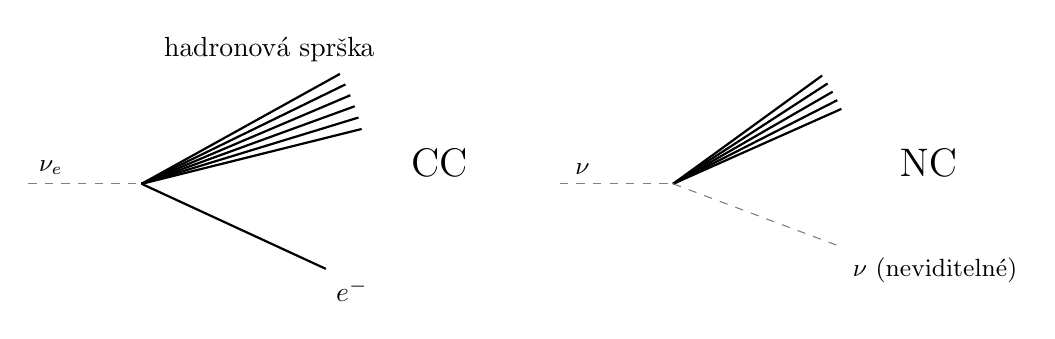
\begin{tikzpicture}[scale=0.9]
  % CC event
  \begin{scope}
    \coordinate (v) at (0,0);
    \draw[dashed,gray] (-1.6,0) -- (v) node[pos=0.2,above,black] {\small \(\nu_e\)};
    \foreach \a in {14,17,20,23,26,29}{
      \draw[thick] (v) -- ++(\a:3.2);
    }
    \draw[thick] (v) -- (2.6,-1.2) node[below right] {\(e^-\)};
    \node at (1.8,1.9) {hadronová sprška};
    \node[font=\Large] at (4.2,0.3) {CC};
  \end{scope}
  % NC event
  \begin{scope}[xshift=7.5cm]
    \coordinate (v) at (0,0);
    \draw[dashed,gray] (-1.6,0) -- (v) node[pos=0.2,above,black] {\small \(\nu\)};
    \foreach \a in {24,27,30,33,36}{
      \draw[thick] (v) -- ++(\a:2.6);
    }
    \draw[dashed,gray] (v) -- (2.4,-0.9) node[below right,black] {\small \(\nu\) (neviditelné)};
    \node[font=\Large] at (3.6,0.3) {NC};
  \end{scope}
\end{tikzpicture}
\end{center}

V události CC vidíme z vrcholu interakce vycházet jednak hadronovou spršku (rozbitý nukleon, resp. kvark, který dostal velký impuls), jednak \emph{nabitý lepton} -- zde elektron \(e^-\). V události NC odchází neutrino neviditelně a v detektoru zbude \emph{jen} hadronová sprška bez leptonu. Počítáním událostí „sprška + lepton“ a „jen sprška“ se oba poměry změří.

\begin{vysvetleni}[Objev neutrálních proudů]
Neutrální proudy byly objeveny v roce 1973 v bublinové komoře Gargamelle v CERN právě hledáním událostí typu „hadrony bez mionu“ ve svazku \(\nu_\mu\). Šlo o první velké potvrzení elektroslabé teorie Glashowa, Weinberga a Salama -- \(Z^0\) samo bylo přímo pozorováno až v roce 1983. V partonovém modelu (izoskalární terč, zanedbání mořských kvarků) platí Llewellyn-Smithovy vztahy
\[
  R_\nu=\frac{\sigma^{NC}_{\nu N}}{\sigma^{CC}_{\nu N}}=\tfrac12-\sin^2\theta_W+\tfrac{20}{27}\sin^4\theta_W\approx 0.31,\qquad
  R_{\bar\nu}=\tfrac12-\sin^2\theta_W+\tfrac{20}{9}\sin^4\theta_W\approx 0.38
\]
pro \(\sin^2\theta_W\approx0.23\). Měření těchto poměrů bylo historicky jedním z prvních způsobů, jak určit Weinbergův úhel.
\end{vysvetleni}

\subsection{Oscilace neutrin}

Zatím jsme mlčky předpokládali, že neutrino, které vzniklo jako \(\nu_e\) (tj. spolu s elektronem nebo pozitronem), zůstane \(\nu_e\) i ve chvíli, kdy po cestě interaguje v detektoru. Experimenty se slunečními a atmosférickými neutriny (viz dále) ale ukázaly, že tomu tak není: neutrino se během letu může „přeměnit“ na jinou vůni. Tento jev se nazývá \kw{oscilace neutrin} a je kvantově-mechanickým důsledkem dvou faktů -- neutrina mají nenulové (a navzájem různé) hmotnosti a stavy s určitou vůní nejsou stavy s určitou hmotností. Ukážeme si to nejprve na zjednodušeném modelu se dvěma vůněmi.

\strana{P10-2}
\begin{itemize}[nosep]
  \item Máme \textbf{dva stavy vůně} \(\nu_e\), \(\nu_\mu\). To jsou stavy, které vznikají a zanikají ve slabé interakci (CC vrchol vždy páruje \(\nu_e\) s \(e\), \(\nu_\mu\) s \(\mu\)).
  \item Máme \textbf{dva hmotové stavy} \(\nu_1\), \(\nu_2\) s hmotnostmi \(m_1\), \(m_2\). To jsou vlastní stavy hamiltoniánu volné částice, tedy stavy, které se šíří prostorem s dobře definovanou energií a hybností.
\end{itemize}
Obě dvojice tvoří ortonormální báze téhož dvourozměrného prostoru,
\[
  \braket{\nu_e}{\nu_\mu}=0,\qquad \braket{\nu_1}{\nu_2}=0,
\]
a jsou tedy navzájem spojeny unitární (zde reálnou ortogonální) maticí, tj. otočením o \kw{směšovací úhel} \(\theta\):
\begin{equation}
  \begin{pmatrix}\nu_e\\ \nu_\mu\end{pmatrix}
  =\begin{pmatrix}\cos\theta & \sin\theta\\ -\sin\theta & \cos\theta\end{pmatrix}
  \begin{pmatrix}\nu_1\\ \nu_2\end{pmatrix}.
\end{equation}
Kdyby bylo \(\theta=0\), splývaly by stavy vůně s hmotovými a žádné oscilace by nenastaly.

\paragraph{Časový vývoj.} Předpokládejme, že v čase \(t=0\) v bodě \(\vec x=0\) vzniklo elektronové neutrino (např. v jaderné reakci ve Slunci). Rozložíme ho do hmotových stavů:
\begin{equation}
  \ket{\psi(0)}=\ket{\nu_e}=\cos\theta\ket{\nu_1}+\sin\theta\ket{\nu_2}.
\end{equation}
Proč právě do hmotových? Protože pouze o nich víme, jak se vyvíjejí: každá složka se šíří jako rovinná vlna se svou energií \(E_j\) a hybností \(\vec p_j\), tj. získává fázový faktor \(e^{-i(E_jt-\vec p_j\cdot\vec x)/\hbar}\). V zápisu z přednášky (energie a hybnosti měříme v energetických jednotkách, tj. \(E_j\) a \(p_j\) znamenají \(E_j\) a \(p_jc\), hmotnosti znamenají \(m_jc^2\)) je
\begin{equation}
  \ket{\psi(\vec x,t)}=\cos\theta\ket{\nu_1}\,e^{-i\frac{E_1tc-\vec p_1\cdot\vec x}{\hbar c}}
  +\sin\theta\ket{\nu_2}\,e^{-i\frac{E_2tc-\vec p_2\cdot\vec x}{\hbar c}}.
\end{equation}
Zavedeme označení fází
\begin{equation}
  \varphi_j\equiv\left(E_j\,t\,c-\vec p_j\cdot\vec x\right)/(\hbar c)\ \longrightarrow\ \frac{1}{\hbar c}\left(E_j\,t\,c-p_j\,x\right)\qquad(\vec p\parallel\vec x),
\end{equation}
kde jsme v posledním kroku využili, že neutrino letí ve směru spojnice zdroj--detektor, takže \(\vec p_j\cdot\vec x=p_jx\). Klíčové je, že pokud \(m_1\neq m_2\), jsou fáze \(\varphi_1\) a \(\varphi_2\) obecně různé -- obě složky „běží“ různě rychle a jejich relativní fáze se během letu mění. Tím se mění i to, jakou superpozici stavů vůně stav \(\ket{\psi}\) představuje.

\paragraph{Pravděpodobnost přeměny \(\nu_e\to\nu_\mu\).} Detektor registruje vůni (např. vznikne-li v CC interakci mion, víme, že dorazilo \(\nu_\mu\)). Pravděpodobnost, že v bodě \(x\) a čase \(t\) najdeme mionové neutrino, je kvadrát průmětu. Z inverze směšovací matice máme \(\bra{\nu_\mu}=-\sin\theta\bra{\nu_1}+\cos\theta\bra{\nu_2}\), a tedy
\begin{align}
  \left|\braket{\nu_\mu}{\psi(\vec x,t)}\right|^2
  &=\Big|\big(-\bra{\nu_1}\sin\theta+\bra{\nu_2}\cos\theta\big)\big(\cos\theta\ket{\nu_1}e^{-i\varphi_1}+\sin\theta\ket{\nu_2}e^{-i\varphi_2}\big)\Big|^2=\notag\\
  &=\left|-\sin\theta\cos\theta\,e^{-i\varphi_1}+\sin\theta\cos\theta\,e^{-i\varphi_2}\right|^2=\notag\\
  &=\sin^2\theta\cos^2\theta\left|-e^{-i\varphi_1}+e^{-i\varphi_2}\right|^2
   =\sin^2\theta\cos^2\theta\left[1+1-2\,\mathrm{Re}\!\left(e^{-i\varphi_1}e^{i\varphi_2}\right)\right]=\notag\\
  &=\tfrac12\sin^22\theta\,(1-\cos\Delta\varphi)
   =\tfrac12\sin^22\theta\left[1-\left(\cos^2\tfrac{\Delta\varphi}{2}-\sin^2\tfrac{\Delta\varphi}{2}\right)\right]=\notag\\
  &=\vzorec{\sin^22\theta\,\sin^2\frac{\Delta\varphi}{2}}.
\end{align}
V druhém řádku jsme využili ortonormalitu \(\braket{\nu_i}{\nu_j}=\delta_{ij}\) (smíšené členy vypadnou), ve třetím rozepsali kvadrát absolutní hodnoty \(|a+b|^2=|a|^2+|b|^2+2\,\mathrm{Re}(a^*b)\) a ve čtvrtém použili \(\sin\theta\cos\theta=\frac12\sin2\theta\) (tedy \(\sin^2\theta\cos^2\theta=\frac14\sin^22\theta\)), \(\Delta\varphi\equiv\varphi_2-\varphi_1\) a \(1-\cos\Delta\varphi=2\sin^2\frac{\Delta\varphi}{2}\).

\strana{P10-3}
Protože se neutrino buď nezměnilo, nebo změnilo (v modelu se dvěma vůněmi jiná možnost není), je pravděpodobnost přežití
\begin{equation}
  \left|\braket{\nu_e}{\psi(\vec x,t)}\right|^2=1-\sin^22\theta\,\sin^2\frac{\Delta\varphi}{2}.
\end{equation}
Výsledek má jasnou strukturu: \(\sin^22\theta\) je \emph{amplituda} oscilací (jak velká část neutrin se maximálně může přeměnit; maximální je pro \(\theta=45^\circ\)) a \(\sin^2(\Delta\varphi/2)\) popisuje, jak se přeměna mění se vzdáleností.

\paragraph{Fázový rozdíl.} Zbývá vyjádřit \(\Delta\varphi\) pomocí měřitelných veličin. Podle definice
\begin{equation}
  \Delta\varphi=\frac{1}{\hbar c}\left(E_2\,c\,t-p_2x\right)-\frac{1}{\hbar c}\left(E_1\,c\,t-p_1x\right).
\end{equation}
Abychom mohli pokračovat, potřebujeme předpoklad o kinematice obou hmotových složek. Učebnicově se uvádějí dvě varianty a obě vedou ke stejnému výsledku:

\emph{a) Stejná hybnost}, \(p\equiv p_1=p_2\). Pak hybnostní členy vypadnou a pro ultrarelativistická neutrina (\(m\ll p\)) rozvineme \(\sqrt{p^2+m^2}\approx p+\frac{m^2}{2p}\):
\begin{align}
  \Delta\varphi&=\frac{1}{\hbar c}\,c\,t\left(\sqrt{p^2+m_2^2}-\sqrt{p^2+m_1^2}\right)
  \doteq\frac{1}{\hbar}\,t\left(p+\frac{m_2^2}{2p}-p-\frac{m_1^2}{2p}\right)=\notag\\
  &=\frac{t\,(m_2^2-m_1^2)}{2p\,\hbar}\ \doteq\ \frac{x\,(m_2^2-m_1^2)}{2E\,\hbar c},
\end{align}
kde jsme v posledním kroku použili, že neutrino letí prakticky rychlostí světla, \(x\approx ct\), a \(p\approx E\).

\emph{b) Stejná energie}, \(E\equiv E_1=E_2\). Pak vypadnou časové členy a liší se hybnosti \(p_j=\sqrt{E^2-m_j^2}\approx E-\frac{m_j^2}{2E}\):
\begin{align}
  \Delta\varphi&=\frac{-1}{\hbar c}\left(\sqrt{E^2-m_2^2}\cdot x-\sqrt{E^2-m_1^2}\cdot x\right)
  =\frac{-1}{\hbar c}\,x\left(E-\frac{m_2^2}{2E}-E+\frac{m_1^2}{2E}\right)=\notag\\
  &=\frac{x\,(m_2^2-m_1^2)}{2E\,\hbar c}.
\end{align}

\begin{vysvetleni}[Proč oba předpoklady dávají totéž]
Ani jeden z předpokladů „stejná hybnost“ či „stejná energie“ není přesně pravdivý -- korektní popis používá vlnová klubka. Rozhodující ale je, že fázový rozdíl je úměrný \(\Delta m^2\) a jakékoli rozumné kinematické předpoklady dávají v ultrarelativistické limitě stejný výsledek \(\Delta\varphi=\Delta m^2\,x/(2E\hbar c)\). Důležité důsledky: (i) oscilace měří \emph{rozdíl kvadrátů hmot} \(\Delta m^2\), ne hmoty samotné; (ii) oscilace jsou funkcí poměru \(L/E\) (vzdálenost/energie), a proto se experimenty charakterizují právě hodnotou \(L/E\).
\end{vysvetleni}

Dosazením \(\Delta\varphi/2=x\,(m_2^2-m_1^2)/(4E\hbar c)\) dostáváme hlavní výsledek:
\begin{veta}[Oscilace dvou vůní neutrin]
\[
  P_{\nu_e\to\nu_e}(x)=1-\sin^22\theta\,\sin^2\!\left(\frac{x\,(m_2^2-m_1^2)}{4E\hbar c}\right),\qquad
  P_{\nu_e\to\nu_\mu}(x)=\sin^22\theta\,\sin^2\!\left(\frac{x\,(m_2^2-m_1^2)}{4E\hbar c}\right).
\]
Zde \(x\) je uražená vzdálenost (často značená \(L\)), \(E\) energie neutrina a \(m_j\) znamená \(m_jc^2\).
\end{veta}
V praktických jednotkách: \(\dfrac{\Delta m^2 x}{4E\hbar c}\approx1.27\,\dfrac{\Delta m^2[\mathrm{eV^2}]\;x[\mathrm{km}]}{E[\mathrm{GeV}]}\). Oscilační délka \(L_{\mathrm{osc}}=4\pi E\hbar c/\Delta m^2\) tak pro \(\Delta m^2\sim10^{-3}\,\mathrm{eV^2}\) a \(E\sim1\,\mathrm{GeV}\) vychází řádově tisíce kilometrů -- proto jsou oscilace v laboratoři nepozorovatelné a k jejich objevu bylo třeba přírodních zdrojů na velké vzdálenosti (Slunce, atmosféra na druhé straně Země).

\subsection{Sluneční neutrina \texorpdfstring{\(\nu_e\)}{nu\_e}}

Ve Slunci probíhá termojaderná fúze (pp-cyklus), v níž se souhrnně čtyři protony mění na \(^4\)He; při přeměně \(p\to n\) vzniká vždy elektronové neutrino. Slunce je tedy intenzivním zdrojem čistých \(\nu_e\) a standardní sluneční model předpovídá jejich tok. Porovnání předpovědi s měřením bylo první indicií oscilací.

\strana{P10-4}
\paragraph{1. Homestake mine (USA, Jižní Dakota), R.~Davis} (1970--1994)
\begin{itemize}[nosep]
  \item Detektor: nádrž s \(615\) tunami tetrachlorethylenu \(\mathrm{C_2Cl_4}\) (běžná čisticí kapalina -- levný zdroj chloru) hluboko pod zemí v dole, aby byl odstíněn od kosmického záření.
  \item Detekční reakce (záchyt neutrina na chloru, inverzní \(\beta\)-proces):
  \[
    \nu_e+{}^{37}\mathrm{Cl}\to{}^{37}\mathrm{Ar}+e^-\qquad(\text{prahová energie }0.814\,\mathrm{MeV}).
  \]
  Práh znamená, že metoda je citlivá jen na energetičtější část slunečních neutrin (hlavně z \(^7\)Be a \(^8\)B), nikoli na nejčetnější nízkoenergetická neutrina z reakce \(pp\).
  \item Vzniklý argon je radioaktivní a rozpadá se záchytem elektronu zpět:
  \[
    e^-+{}^{37}\mathrm{Ar}\to{}^{37}\mathrm{Cl}+\nu_e,\qquad T_{1/2}=\oprava{35}{34}\ \text{dní}.
  \]
  Postup: argon (vzácný plyn) se každých několik týdnů z nádrže vyplachoval heliem, a jednotlivé atomy \(^{37}\)Ar se počítaly pomocí jejich rozpadů v malém proporcionálním počítači. Poločas o délce měsíce je ideální -- atomy se stihnou nahromadit, ale zároveň se rozpadnou v rozumné době při počítání.
  \item Očekávali \(1.7\) interakcí za den, naměřili \(0.48\) interakcí za den -- tedy jen asi třetinu předpovědi. To je tzv. \kw{problém slunečních neutrin}. Nebylo jasné, zda je chyba v experimentu, ve slunečním modelu, nebo v neutrinech samotných.
\end{itemize}

\paragraph{2. SNO -- Sudbury Neutrino Observatory (Kanada)} (1999--2006)

Rozhodující krok byl umět změřit zároveň tok \(\nu_e\) a celkový tok neutrin všech vůní. SNO \textbf{uměl rozlišit \(\nu_e\) od ostatních vůní}. Detektorem bylo \(1000\) tun těžké vody \(\mathrm{D_2O}\), tj. \(\left({}^2_1\mathrm{H}\right)_2\mathrm{O}\). Deuteron je slabě vázaný, takže na něm mohou proběhnout dvě různé reakce:
\begin{itemize}[nosep]
  \item \textbf{nabité proudy} (jen \(\nu_e\), protože sluneční neutrina nemají dost energie na vytvoření \(\mu\) či \(\tau\)):
  \[
    \nu_e+{}^2_1\mathrm{H}\to p+p+e^-,
  \]
  rychlý elektron vyzařuje \kw{Čerenkovovo záření} (ČZ), které registrují fotonásobiče na stěnách nádoby;
  \item \textbf{neutrální proudy} (stejně pro všechny vůně \(\nu_x\), \(x=e,\mu,\tau\)):
  \[
    \nu_x+{}^2_1\mathrm{H}\to p+n+\nu_x .
  \]
  Neutrino zde jen rozbije deuteron (práh \(2.2\,\mathrm{MeV}\) = vazebná energie deuteronu). Volný neutron je třeba zaregistrovat; k tomu se do vody přidala kuchyňská sůl NaCl a neutron se zachytí na chloru:
  \[
    n+{}^{35}\mathrm{Cl}\to{}^{36}\mathrm{Cl}^*\to{}^{36}\mathrm{Cl}+\gamma ,
  \]
  vzniklá fotonová kaskáda (\(\approx8.6\,\mathrm{MeV}\)) se opět detekuje přes Čerenkovovo záření elektronů, které fotony vyrazí.
\end{itemize}
Zastoupení izotopů chloru v přírodě: \(^{35}\)Cl: \(\oprava{75}{25}\,\%\), \(^{37}\)Cl: \(\oprava{25}{75}\,\%\). (\(^{35}\)Cl má navíc velký účinný průřez pro záchyt tepelných neutronů, asi \(44\,\mathrm{b}\), proto je pro detekci neutronů výhodný.)

\begin{veta}[Výsledek SNO]
Tok \(\nu_e\) (z CC) je jen \(\approx\frac13\) očekávaného, \textbf{ale celkový tok neutrin} (z NC, všechny vůně) \textbf{je správně} -- souhlasí se slunečním modelem. Neutrina tedy ze Slunce nemizí, jen se cestou mění:
\[
  \nu_e\to\nu_x\quad(x=\mu,\tau).
\]
\end{veta}
Tím byl problém slunečních neutrin vyřešen: sluneční model byl správný a chybějící \(\nu_e\) se přeměnily na \(\nu_\mu\) a \(\nu_\tau\), které v Homestake (ani v CC kanálu SNO) nebylo možné vidět (viz Davídkovy slajdy „Oscilace neutrin (1)--(3)“).

\begin{vysvetleni}[Proč právě jedna třetina]
Naivně by se mohlo zdát, že při průměrování přes mnoho oscilací by mělo zbýt \(1-\frac12\sin^22\theta\). Pro energetická \(^8\)B neutrina, na která je SNO citlivý, však hraje roli i interakce s elektrony v hustém nitru Slunce (\kw{MSW efekt}): neutrino opouští Slunce prakticky v čistém hmotovém stavu \(\nu_2\), a pravděpodobnost, že bude detekováno jako \(\nu_e\), je pak \(|U_{e2}|^2\approx\sin^2\theta_{12}\approx0.3\), tedy zhruba třetina. Podrobný výklad jde nad rámec přednášky.
\end{vysvetleni}

\strana{P10-5}
\subsection{Atmosférická neutrina}

Druhým přírodním zdrojem jsou \kw{atmosférická neutrina}. Primární kosmické záření (převážně protony) naráží do horní atmosféry (ve výšce \(\sim15\,\mathrm{km}\)) a vytváří piony, které se rozpadají:
\[
  \pi^\pm\to\mu^\pm+\overset{(-)}{\nu}_{\!\mu},\qquad
  \mu^\pm\to e^\pm+\overset{(-)}{\nu}_{\!\mu}+\overset{(-)}{\nu}_{\!e}.
\]
\begin{itemize}[nosep]
  \item \textbf{Malé energie} (\(E_\nu\lesssim1\,\mathrm{GeV}\)): z jednoho pionu vzniknou celkem dvě mionová a jedno elektronové (anti)neutrino, takže
  \[
    \frac{\nu_\mu+\bar\nu_\mu}{\nu_e+\bar\nu_e}\approx2.
  \]
  \item \textbf{Vyšší energie} \(\to\) poměr roste. Rychlé miony mají díky dilataci času tak dlouhou dobu života, že často doletí až na zem a zastaví se dřív, než se ve vzduchu rozpadnou -- elektronová neutrina z jejich rozpadu pak chybí.
\end{itemize}
Tento poměr je teoreticky dobře spočitatelný (na rozdíl od absolutního toku), proto se odchylky od něj dají spolehlivě interpretovat.

\paragraph{Detekce (Super-Kamiokande, Japonsko).} Obrovský vodní detektor (\(50\,000\) t vody) s fotonásobiči detekuje Čerenkovovo záření leptonů z CC interakcí
\[
  \nu_\mu+n\to p+\mu^-,\qquad \nu_e+n\to p+e^-.
\]
Mion vytvoří ostrý Čerenkovův prstenec, elektron rozmazaný (elektron vyvolá elmag.\ spršku), takže detektor umí rozlišit \(\nu_\mu\) od \(\nu_e\). Ze směru leptonu se navíc určí přibližný směr příletu neutrina, tedy \kw{zenitový úhel}.

\begin{center}
\begin{tikzpicture}[scale=1]
  \draw[thick] (0,0) circle (2);
  \node at (-1.2,0.2) {Země};
  % detektor
  \fill[pattern=north east lines] (-0.18,1.72) rectangle (0.18,2.02);
  \draw (-0.18,1.72) rectangle (0.18,2.02);
  % down-going
  \foreach \dx in {-0.35,-0.15,0.05,0.25}{
    \draw[-{Stealth[length=2mm]}] (\dx*1.6,3.6) -- (\dx*0.2,2.08);
  }
  \node[right] at (0.5,3.5) {\(\nu_\mu\)};
  \node[right] at (0.9,2.9) {Down};
  \node[right,ForestGreen] at (0.9,2.45) {\(\sim10\,\mathrm{km}\)};
  % up-going (through Earth)
  \draw[-{Stealth[length=2mm]}] (-1.0,-2.6) -- (-0.05,1.7);
  \draw[-{Stealth[length=2mm]}] (0.05,-2.6) -- (0.0,1.7);
  \draw[-{Stealth[length=2mm]}] (0.6,-2.6) -- (0.05,1.7);
  \node[right] at (1.0,-2.3) {Up};
  \node[right,ForestGreen] at (1.6,-2.3) {\(\sim10^4\,\mathrm{km}\)};
\end{tikzpicture}
\end{center}

Klíčová myšlenka: neutrina přilétající shora („Down“) urazí jen tloušťku atmosféry, \(\sim10\,\mathrm{km}\); neutrina přilétající zespodu („Up“) prolétla celou Zemí, \(\sim10^4\,\mathrm{km}\) (průměr Země je \(12\,700\,\mathrm{km}\)). Země je pro neutrina prakticky průhledná a tok kosmického záření je izotropní, takže \emph{bez oscilací} by tok shora a zdola musel být stejný. Super-Kamiokande (1998) změřil asymetrii mionových neutrin (s \(E\gtrsim1\,\mathrm{GeV}\))
\begin{equation}
  A=\frac{U-D}{U+D}=-0.296\pm0.048\,(\text{stat.})\pm\oprava{0.01}{0.001}\,(\text{syst.}),
\end{equation}
tedy neutrin zdola (s dlouhou dráhou) je výrazně méně. Elektronová neutrina žádnou takovou asymetrii nevykazovala, proto se \(\nu_\mu\) mění převážně na \(\nu_\tau\) (které SK při těchto energiích nedetekuje). Šlo o první přesvědčivý důkaz oscilací neutrin (Nobelova cena 2015, T.~Kajita, spolu s A.~McDonaldem za SNO).

\paragraph{Určení \(\Delta m^2\).} SK měřil úbytek \(\nu_\mu\) v závislosti na zenitovém úhlu, tj. na vzdálenosti \(x\), a na energii -- tedy jako funkci \(x/E\). Pravděpodobnost přežití
\[
  P_{\nu_\mu\to\nu_\mu}=1-\sin^22\theta\,\sin^2\!\left(\frac{x\,\Delta m^2}{4\hbar cE}\right)
\]
má \textbf{minimum při \(x/E\approx500\,\mathrm{km/GeV}\)}.

\strana{P10-6}
První minimum nastane, když je argument sinu roven \(\pi/2\):
\[
  \frac{\pi}{2}=\frac{\Delta m^2}{4\hbar c}\cdot\frac{500\,\mathrm{km}}{1\,\mathrm{GeV}} .
\]
\begin{priklad}[Odhad \(\Delta m^2_{23}\) z atmosférických neutrin]
Vyjádříme \(\Delta m^2\) a dosadíme \(\hbar c\approx200\,\mathrm{MeV\,fm}\), \(1\,\mathrm{GeV}=1000\,\mathrm{MeV}\), \(500\,\mathrm{km}=500\times10^3\times10^{15}\,\mathrm{fm}\):
\begin{align*}
  \Delta m^2&=2\hbar c\pi\,\frac{1\,\mathrm{GeV}}{500\,\mathrm{km}}
  =\frac{2\pi\cdot200\,\mathrm{MeV\,fm}}{1}\cdot\frac{1000\,\mathrm{MeV}}{500\times10^3\times10^{15}\,\mathrm{fm}}=\\
  &=8\pi\cdot10^{-16}\,\mathrm{MeV^2}\approx25\cdot10^{-4}\,\mathrm{eV^2}=\vzorec{2.5\cdot10^{-3}\,\mathrm{eV^2}}.
\end{align*}
(\(1\,\mathrm{MeV^2}=10^{12}\,\mathrm{eV^2}\); \(\Delta m^2\) zde znamená \(\Delta(m^2c^4)\).) Rozdíl kvadrátů hmot je tedy nepatrný -- kdyby byla jedna z hmot nulová, ta druhá by byla \(\sqrt{2.5\cdot10^{-3}}\,\mathrm{eV}\approx0.05\,\mathrm{eV}\). To je v souladu s přímými limitami z \(\beta\)-rozpadu tritia (\(m_{\nu_e}<0.45\,\mathrm{eV}\), KATRIN).
\end{priklad}

Navíc bylo pozorováno, že v minimu je úbytek maximální možný: kdyby minimum bylo \(P_{\nu_\mu\to\nu_\mu}=0\), plyne
\[
  \Rightarrow\quad \sin^22\theta=1,\qquad \sin2\theta=1,\qquad \vzorec{\theta=45^\circ}.
\]
Atmosférický směšovací úhel \(\theta_{23}\) je tedy (téměř) maximální -- \(\nu_\mu\) a \(\nu_\tau\) jsou „rovnoměrnými“ směsmi hmotových stavů \(\nu_2,\nu_3\).

\begin{vysvetleni}[Průběh pravděpodobnosti přežití]
Pro \(\theta=45^\circ\) a \(\Delta m^2=2.5\cdot10^{-3}\,\mathrm{eV^2}\) vypadá \(P_{\nu_\mu\to\nu_\mu}\) jako funkce \(x/E\) takto:
\begin{center}
\begin{tikzpicture}[xscale=0.5,yscale=2.2]
  \draw[-{Stealth}] (0,0) -- (21,0) node[above left] {\small \(x/E\) [km/GeV]};
  \draw[-{Stealth}] (0,0) -- (0,1.25) node[left] {\small \(P_{\nu_\mu\to\nu_\mu}\)};
  \foreach \t in {0,5,10,15,20}{ \draw (\t,0) -- (\t,-0.04) node[below] {\scriptsize \pgfmathparse{int(\t*100)}\pgfmathresult}; }
  \draw (0,1) -- (-0.2,1) node[left] {\scriptsize 1};
  \draw[thick,vysvbarva,domain=0:20,samples=200] plot (\x,{1-(sin(0.3168*\x r))^2});
  \draw[dashed,gray] (4.96,0) -- (4.96,1.1) node[above,black] {\scriptsize \(\approx500\)};
\end{tikzpicture}
\end{center}
V reálném experimentu se díky rozmazání v energii a směru rychlé oscilace pro velké \(x/E\) zprůměrují k hodnotě \(1-\frac12\sin^22\theta=\frac12\) -- proto neutrin zdola chybí zhruba polovina, zatímco neutrina shora (\(x/E\) malé) ještě oscilovat nestihla. (Srv.\ Davídkovy slajdy „Oscilace neutrin (5)“.)
\end{vysvetleni}

\subsection{Popis pro 3 rodiny neutrin}

Ve skutečnosti existují tři vůně neutrin (\(\nu_e,\nu_\mu,\nu_\tau\); počet lehkých neutrin \(N_\nu\approx3\) změřil LEP z šířky \(Z^0\)) a tedy i tři hmotové stavy. Směšovací matice je \(3\times3\) unitární matice, zvaná \kw{PMNS matice} (Pontecorvo--Maki--Nakagawa--Sakata), obdoba CKM matice v kvarkovém sektoru:
\begin{equation}
  \begin{pmatrix}\nu_e\\ \nu_\mu\\ \nu_\tau\end{pmatrix}
  =\begin{pmatrix}U_{e1}&U_{e2}&U_{e3}\\ U_{\mu1}&U_{\mu2}&U_{\mu3}\\ U_{\tau1}&U_{\tau2}&U_{\tau3}\end{pmatrix}
  \begin{pmatrix}\nu_1\\ \nu_2\\ \nu_3\end{pmatrix}
  \qquad\text{(PMNS)}.
\end{equation}
Obecná unitární matice \(3\times3\) má po odečtení nefyzikálních fází \textbf{tři úhly a jednu fázi} \(\delta\) (narušující CP symetrii). Standardní parametrizace je součin tří rotací:
\begin{equation}
  U=\begin{pmatrix}1&0&0\\0&\cos\theta_{23}&\sin\theta_{23}\\0&-\sin\theta_{23}&\cos\theta_{23}\end{pmatrix}
  \begin{pmatrix}\cos\theta_{13}&0&\sin\theta_{13}\,e^{-i\delta}\\0&1&0\\-\sin\theta_{13}\,e^{i\delta}&0&\cos\theta_{13}\end{pmatrix}
  \begin{pmatrix}\cos\theta_{12}&\sin\theta_{12}&0\\-\sin\theta_{12}&\cos\theta_{12}&0\\0&0&1\end{pmatrix}.
\end{equation}
Výhoda této parametrizace je v tom, že jednotlivé matice přibližně odpovídají jednotlivým typům experimentů: první rotace (\(\theta_{23}\)) „atmosférická“, poslední (\(\theta_{12}\)) „sluneční“ a prostřední (\(\theta_{13}\), s fází \(\delta\)) „reaktorová“. Protože jsou dva rozdíly \(\Delta m^2\) velmi odlišné, lze v každém experimentu oscilace přibližně popsat dvouvůňovým vzorcem odvozeným výše s příslušným úhlem a \(\Delta m^2\).

\strana{P10-7}
Naměřené hodnoty:
\begin{itemize}[nosep]
  \item \textbf{sluneční neutrina} (\(\nu_e\to\nu_{\mu,\tau}\)):
  \(\Delta m^2_{12}\approx-7.5\cdot10^{-5}\,\mathrm{eV^2}\), \quad \(\theta_{12}\approx34^\circ\);
  \item \textbf{atmosférická neutrina} (\(\nu_\mu\to\nu_\tau\)):
  \(|\Delta m^2_{23}|\approx2.5\cdot10^{-3}\,\mathrm{eV^2}\) (náš odhad výše), \(\theta_{23}\approx45^\circ\);
  \item \textbf{úhel \(\theta_{13}\) je malý} (změřen až reaktorovými experimenty, Daya Bay 2012: \(\theta_{13}\approx8.5^\circ\)).
\end{itemize}
Znaménková konvence je zde \(\Delta m^2_{12}\equiv m_1^2-m_2^2\) (jako na Davídkových slajdech), záporná hodnota tedy znamená \(m_2>m_1\). Znaménko je známo díky MSW efektu ve Slunci, zatímco atmosférické oscilace ve vakuu jsou citlivé jen na \(|\Delta m^2_{23}|\).

\begin{vysvetleni}[Co zatím nevíme]
\begin{itemize}[nosep,leftmargin=*]
  \item \kw{Hierarchie hmot}: buď \(m_1<m_2<m_3\) (normální), nebo \(m_3<m_1<m_2\) (inverzní) -- znaménko \(\Delta m^2_{23}\) zatím není spolehlivě určeno.
  \item Absolutní škála hmot -- oscilace měří jen rozdíly kvadrátů; přímé měření (KATRIN) dává jen horní mez.
  \item Velikost CP-narušující fáze \(\delta\) -- měří se porovnáním oscilací \(\nu_\mu\to\nu_e\) a \(\bar\nu_\mu\to\bar\nu_e\) na urychlovačích (T2K, NOvA, budoucí DUNE, Hyper-Kamiokande). Mohla by souviset s asymetrií hmoty a antihmoty ve vesmíru.
  \item Zda jsou neutrina Diracovy, nebo Majoranovy částice (tj. zda je neutrino svou vlastní antičásticí) -- hledá se pomocí bezneutrinového dvojitého \(\beta\)-rozpadu.
\end{itemize}
Viz Davídkovy slajdy „Oscilace neutrin (6)--(8)“ a „Otevřené otázky částicové fyziky“.
\end{vysvetleni}
